\subsubsection{Kalibracja kamery}
Do uruchomienia algorytmu potrzebny jest plik kalibracyjny. Kalibracj� kamery wykonano standardowym narz�dziem zaimplementowanym w ROSie w paczce  \texttt{camera\_calibration}. Wynikiem tej operacji jest plik *.yml. Na potrzeby algorytmu przkonwertowano plik *.yml na format *.yaml.

\begin{figure}[h!]
\centering
	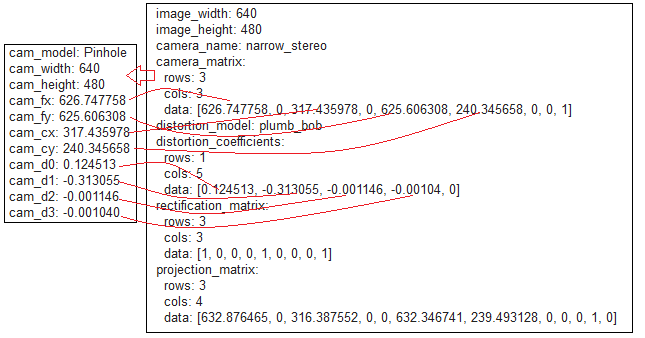
\includegraphics[scale=0.6]{grafika/kali.png}
	\caption{Konwersja pliku *.yml na *.yaml}
	\label{yml}
\end{figure}
Rysunek \ref{yml} przedstawia r�czne przekonwertowanie pliku kalibracyjne.
\subsubsection{Rezultat algorytmu}
Do dalszego przetwarzania informacji dostarczonych z dzia�aj�cej paczki SVO mo�na wykorzysta� wiadomo�� publikowan� poprzez topic \texttt{/svo/points}.
\begin{figure}
\centering
	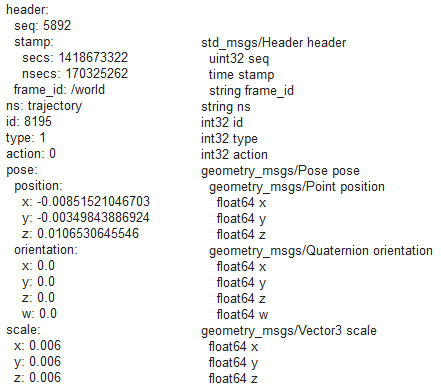
\includegraphics[scale=0.6]{grafika/topic.png}
	\caption{Wycinek informacji zawartych w topicu \texttt{/svo/points}}
	\label{t}
\end{figure}
Rysunek \ref{t} pokazuje struktur� kluczowego topicu SVO. ...